\documentclass[mathserif,18pt,xcolor=table]{beamer}

\usepackage {bbm}
\usepackage {textpos}
\usepackage{tikz}
\usepackage{hyperref}
\usepackage{color}
\usepackage{amsmath}
\usepackage{amssymb}
\usepackage{soul}
\usepackage[compatibility=false]{caption}
\usepackage{subcaption}
\usepackage{multimedia}
\usepackage{multirow}



\definecolor{utorange}{RGB}{203,96,21}
\definecolor{utblack}{RGB}{99,102,106}
\definecolor{utbrown}{RGB}{110,98,89}
\definecolor{utsecbrown}{RGB}{217,200,158}
\definecolor{utsecgreen}{RGB}{208,222,187}
\definecolor{utsecblue}{RGB}{127,169,174}

\newcommand{\norm}[1]{\left\lVert #1 \right\rVert}

\mode<presentation>
{
  % \usetheme{Pittsburgh}   
  \usetheme{Boadilla}  
  \usefonttheme[onlymath]{serif}

  \setbeamercovered{invisible}
  \setbeamertemplate{navigation symbols}{}

  % Color Theme 
    \setbeamercolor{normal text}{bg=white,fg=utblack}
  \setbeamercolor{structure}{fg=utorange}

  \setbeamercolor{alerted text}{fg=red!85!black}

  \setbeamercolor{item projected}{use=item,fg=black,bg=item.fg!35}

  \setbeamercolor*{palette primary}{use=structure,fg=white, bg=utorange}
  \setbeamercolor*{palette secondary}{use=structure,bg=utsecbrown}
  \setbeamercolor*{palette tertiary}{use=structure,bg=utsecgreen}
  \setbeamercolor*{palette quaternary}{use=structure,fg=structure.fg,bg=utsecblue}

  % \setbeamercolor*{frametitle}{use=structure,fg=utorange, bg=utsecbrown}
  \setbeamercolor*{framesubtitle}{fg=utbrown}

  \setbeamercolor*{block title}{parent=structure,fg=black,bg=utsecgreen}
  \setbeamercolor*{block body}{fg=black,bg=utblack!10}
  \setbeamercolor*{block title alerted}{parent=alerted text,bg=black!15}
  \setbeamercolor*{block title example}{parent=example text,bg=black!15}

  \setbeamerfont{framesubtitle}{size=\small}
}

\usepackage[orientation=landscape,size=custom,width=16,height=9.75,scale=0.5,debug]{beamerposter}
% \usepackage[orientation=landscape,size=custom,width=16,height=9,scale=0.5,debug]{beamerposter}


\makeatletter
\setbeamertemplate{footline}
{
  \leavevmode%
    \hbox{%
      \begin{beamercolorbox}[wd=.333333\paperwidth,ht=2.25ex,dp=1ex,center]{author in head/foot}%
        \usebeamerfont{author in head/foot}\insertshortauthor%~~\beamer@ifempty{\insertshortinstitute}{}{(\insertshortinstitute)}
      \end{beamercolorbox}%
        \begin{beamercolorbox}[wd=.5\paperwidth,ht=2.25ex,dp=1ex,center]{title in head/foot}%
        \usebeamerfont{title in head/foot}\insertshorttitle
        \end{beamercolorbox}%
        \begin{beamercolorbox}[wd=.166666\paperwidth,ht=2.25ex,dp=1ex,right]{date in head/foot}%
        \usebeamerfont{date in head/foot}\insertshortdate{}\hspace*{2em}
        \insertframenumber{} / \inserttotalframenumber\hspace*{2ex} 
      \end{beamercolorbox}}%
        \vskip0pt%
}
\makeatother

\usepackage{kerkis}
\usepackage[T1]{fontenc}
\usepackage[protrusion=true,expansion=true]{microtype}
\usepackage{amsmath}


\renewcommand*{\thefootnote}{\fnsymbol{footnote}}


\pgfdeclareimage[height=1.0cm]{utbig}{logos/UTWordmark.pdf}
\pgfdeclareimage[height=0.6cm]{ut}{logos/UTWordmark.pdf}

\title{Compressed Sensing: Incoherence and Structured Random Matrices}
\subtitle{Subtitle?}
\author[Keith Kelly, Sameer~Tharakan, Yerlan~Amanbek]{ {Keith~Kelly, Sameer~Tharakan, Yerlan~Amanbek} \\  
}

\institute{Institute for Computational Engineering \& Sciences\\ \mbox{}  \\  \pgfuseimage{utbig} }
\date[ACHA]

\begin{document}

\tikzstyle{block} = [rectangle, draw, rounded corners, shade, top color=white, text width=5em,
  bottom color=blue!50!black!20, draw=blue!40!black!60, very thick, text centered, minimum height=4em]
  \tikzstyle{line} = [draw, -latex']
  \tikzstyle{cloud} = [draw, ellipse,top color=white, bottom color=red!20, node distance=2cm, minimum height=2em]


  \beamertemplateballitem
  %\beamertemplatetransparentcoveredhigh

  \frame{\titlepage}

  \addtobeamertemplate{frametitle}{}{%
      \begin{textblock*}{100mm}(0.95\textwidth,-0.75cm)
    \pgfuseimage{ut}
    \end{textblock*}
  }


% ------------------------------------------------------------
\begin{frame}[t]
\frametitle{Intro}
\framesubtitle{~~}  %% needed for proper positioning of the logo ...

Slides online at

\href{http://users.ices.utexas.edu/~keith/}{\textcolor{blue}{http://users.ices.utexas.edu/\textasciitilde keith/}}


\end{frame}

%%%%%%%%%%%%%%%%%%%%%%%%%%%%%%%%%%%%%%
%% Frame
%%%%%%%%%%%%%%%%%%%%%%%%%%%%%%%%%%%%%%

\begin{frame}[t]
	\frametitle{Introduction}
	\framesubtitle{~~}  %% needed for proper positioning of the logo ...

	The Basis pursuit problem 
	\begin{equation}
		\min ||x||_{l_1} \quad \text{ subject to } \quad \Phi \Psi x=y
	\end{equation}

	\small
	Where $\Psi$ is an $n \times n$ orthogonal matrix corresponding to the basis in which our signal $z = \Psi x$ is $S$-sparse. $\Phi$ is our sensing matrix. 
	\\
	\normalfont
	\textbf{Toeplitz} and \textbf{Circulant} matrices have the forms, respectively,
	\\
	
	$$
	T = \begin{bmatrix}
		t_{1}    & t_{2}    & ...    & t_{n}   \\[0.3em]
		t_{n+1}  & t_{1}    & ...    & t_{n-1} \\[0.3em]
		\ddots   & \ddots   & \ddots &         \\[0.3em]
		t_{2n-1} & t_{2n-2} & ...    & t_{1}         
	\end{bmatrix}
	\qquad \text{and} \qquad
	C = \begin{bmatrix}
		t_{1}  & t_{2}  & ...    & t_{n}   \\[0.3em]
		t_{n}  & t_{1}  & ...    & t_{n-1} \\[0.3em]
		\ddots & \ddots & \ddots &         \\[0.3em]
		t_{2}  & t_{3}  & ...    & t_{1}        
	\end{bmatrix} 
	$$
\end{frame}
%%%%%%%%%%%%%%%%%%%%%%%%%%%%%%%%%%%%%
%% Frame
%%%%%%%%%%%%%%%%%%%%%%%%%%%%%%%%%%%%%%
\begin{frame}[t]
	\frametitle{Structured random matrices}
	\framesubtitle{~~}  %% needed for proper positioning of the logo ...
	Any Circulant matrix can be diagonalized by a Fourier transform, i.e. obeying
	$$ C=\frac{1}{\sqrt{n}} F^* \Sigma F $$ with $F$ as the discrete Fourier matrix
	$F_{t,w}=e^{-i\; 2\pi(t-1)(w-1)/n}, \qquad 1 \le t,w \le n$
	$$
	\Sigma = \begin{bmatrix}
		\sigma_{1} & 0 & ...& 0           \\[0.3em]
		0 & \sigma_{2} & ... & 0 \\[0.3em]
		\ddots &\ddots & \ddots &      \\[0.3em]
		0 & 0 & ... & \sigma_{n}        
	\end{bmatrix} $$
	a diagonal matrix whose entries are unit magnitude complex numbers with random phases.
\end{frame}


%%%%%%%%%%%%%%%%%%%%%%%%%%%%%%%%%%%%%
%% Frame
%%%%%%%%%%%%%%%%%%%%%%%%%%%%%%%%%%%%%%
\begin{frame}[t]
	\frametitle{Structured random matrices}
	\framesubtitle{~~}  %% needed for proper positioning of the logo ...
	We generate $\sigma_{w}$ as follows:
	\\[1em]

	$w=1\qquad \qquad \qquad : \; \sigma_{1} \sim \pm$ 1 with equal probability,
	\\[1em]
	$2 \le w < n/2+1 \; \; : \; \sigma_{w}=e^{i\theta w}, where \; {\theta}_{w} \sim Uniform(0,2\pi) $
	\\[1em]
	$w=n/2+1 \qquad \; \; \, : \; \sigma_{n/2+1} \sim \pm 1 $ with equal probability 
	\\[1em]

	$n/2+2 \le w \le n \; \; : \; \sigma_{w}=\sigma^{*}_{n-w+2}$, conjugate of  $\sigma_{n-w+2}$.
	
	$$
	$$
	Generating the diagonal in this way ensures the resulting circulant matrix is real-valued due 
	to conjugate symmetry.
\end{frame}

%%%%%%%%%%%%%%%%%%%%%%%%%%%%%%%%%%%%%%
%% Frame
%%%%%%%%%%%%%%%%%%%%%%%%%%
%%%%%%%%%%%%
\begin{frame}[t]
	\frametitle{Structured random matrices}
	\framesubtitle{~~}  %% needed for proper positioning of the logo ...
	$$
	T_{n} = \left[ \: 
		\begin{array}{*{4}{c}}
			\cline{1-4}
			\multicolumn{1}{|c}{t_{1}} & t_{2} & ...& \multicolumn{1}{c|}{t_{n}}           \\[0.3em]
			\cline{1-4}
			t_{n+1} & t_{1} & ... & t_{n-1} \\[0.3em]
			\ddots &\ddots & \ddots &    \\[0.3em]
			t_{2n-1} & t_{2n-2} & ... & t_{1}      \\[0.3em]    
		\end{array}
	\right]
	=
	\left[ \:
		\begin{array}{*{4}{c}}
			t_{1} & t_{2} & ...& t_{n}        \\[0.3em]
			\cline{1-1}
			\multicolumn{1}{|c|}{t_{n+1}} & t_{1} & ... & t_{n-1} \\[0.3em]
			\multicolumn{1}{|c|}{\ddots} & \ddots & \ddots &    \\[0.3em]
			\multicolumn{1}{|c|}{t_{2n-1}} & t_{2n-2} & ... & t_{1}          \\[0.3em]
			\cline{1-1}
		\end{array}
	\right]
	$$
	\\
	$$
	C_{2n} =\begin{bmatrix}
		t_{1}   & t_{2} & ...    & t_{n}  & 0   & t_{2n-1} & ... &  t_{n+1}   \\[0.3em]
		t_{n+1} & t_{1} & ...    & t_{n-1}& ... & 0  & ... &          \\[0.3em]
		\ddots  &       & \ddots &        & \ddots & & &\ddots    \\[0.3em]
		\cdots  &       & \cdots &       & \cdots & & & \cdots
	\end{bmatrix}
	=
	\begin{bmatrix}
		T_{n} & B_{n}            \\[0.3em]
		B_{n} & T_{n}   
	\end{bmatrix}
	$$

\end{frame}

%%%%%%%%%%%%%%%%%%%%%%%%%%%%%%%%%%%%%
%% Frame
%%%%%%%%%%%%%%%%%%%%%%%%%%%%%%%%%%%%%%
\begin{frame}[t]
	\frametitle{Structured random matrices}
	\framesubtitle{~~}  %% needed for proper positioning of the logo ...
	\textbf{Hadamard} matrix is a square matrix whose entries are either $+1$ or $-1$ and whose rows are mutually orthogonal.
	\begin{figure}[h]
		\centering
		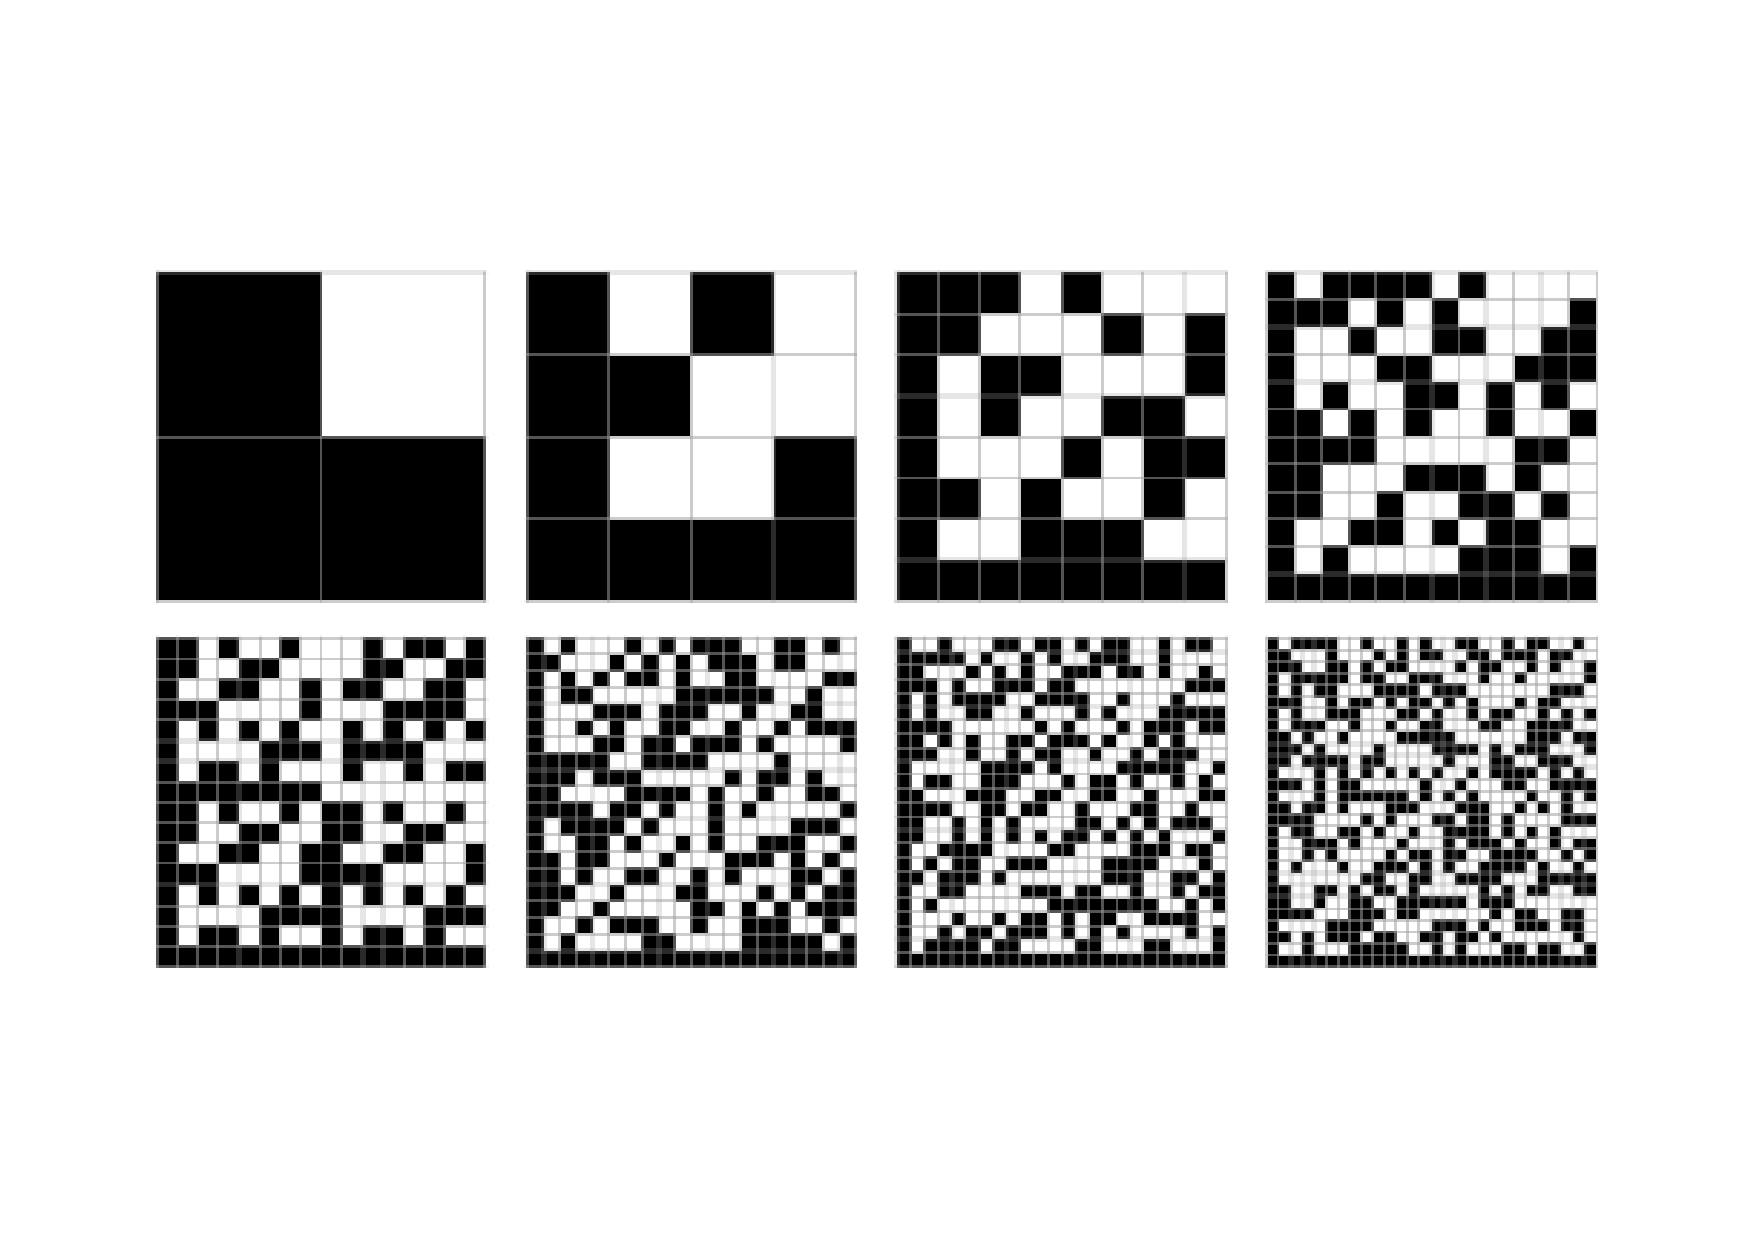
\includegraphics[width=0.7\linewidth]{HadamardMatrices_800}
		\caption{}
		\label{fig:HadamardMatrices_800}
	\end{figure}

\end{frame}
%%%%%%%%%%%%%%%%%%%%%%%%%%%%%%%%%%%%%%
%% Frame
%%%%%%%%%%%%%%%%%%%%%%%%%%%%%%%%%%%%%%
\begin{frame}[t]
	\frametitle{Structured random matrices}
	\framesubtitle{~~}  %% needed for proper positioning of the logo ...
	An equivalent definition of the Hadamard matrices is given by 
	$$ H_{n} H_{n}^T = n  I_{n} $$
	where $I_{n}$ is the $n \times n$ identity matrix.
	$$
	H_{1} = \begin{bmatrix}
		1
	\end{bmatrix}
	\qquad
	H_{2} = \begin{bmatrix}
		1 & 1           \\[0.3em]
		1& -1
	\end{bmatrix}	
	\qquad
	H_{4} = \begin{bmatrix}
		H_{2} & H_{2}           \\[0.3em]
		H_{2}& -H_{2}
	\end{bmatrix}	
	$$
	$$
	\centering
	\qquad
	H_{2^{n}} = \begin{bmatrix}
		H_{2^{n-1}} & H_{2^{n-1}}           \\[0.3em]
		H_{2^{n-1}}& -H_{2^{n-1}}            
	\end{bmatrix}	
	$$
\end{frame}



%%%%%%%%%%%%%%%%%%%%%%%%%%%%%%%%%%%%%%
%% Frame
%%%%%%%%%%%%%%%%%%%%%%%%%%%%%%%%%%%%%%

\begin{frame}[t]
	\frametitle{Structured Random Matrices and the DFR Framework}
	\framesubtitle{~~}  %% needed for proper positioning of the logo ...

	Do et al. (2012) introduced the structured random matrix framework for compressed sensing,
	which is a way of generating sensing matrices $\Phi$ that are incoherent with any basis $\Psi$. Let 

	\centering
	$	\Phi = \sqrt{\frac{N}{M}}DFR$

	\begin{itemize}
	\item $D\in \mathbb{R}^{M\times N}$ (output randomizer) is a subsampling matrix/operator which does one of the following:
		\begin{itemize}
		\item Randomly selects a subset of the entries of a vector (and possibly permutes it) We call this subsampling.
		\item Randomly pre-modulated summation operator as introduced in Romberg, 2008.
		\end{itemize}
	\item $F\in\mathbb{R}^{N\times N}$ is an orthonormal matrix. We usually use a fast transform like the FFT or 
		fast Walsh-Hadamard transform for this.
	\item $R\in\mathbb{R}^{N\times N}$ (input randomizer) is one of the following:
		\begin{itemize}
			\item A uniform random permutation matrix
			\item A diagonal matrix whose entries are Bernoulli random variables with probability $1/2$
		\end{itemize}
	\end{itemize}

\end{frame}

%%%%%%%%%%%%%%%%%%%%%%%%%%%%%%%%%%%%%%
%% Frame
%%%%%%%%%%%%%%%%%%%%%%%%%%%%%%%%%%%%%%
\begin{frame}[t]
	\frametitle{Randomly pre-modulated summation (RPMS)}
	\framesubtitle{~~}  %% needed for proper positioning of the logo ...
	
	Within the DFR framework one, of the restruction or subsampling operators is the
	randomly pre-modulated summation operator. It works as follows:

	Given two vectors $x$ and $\epsilon$, we compute
	\begin{equation}
		y_k = \sqrt{\frac{M}{N}}\sum_{t\in B_k}\epsilon_t x_t
	\end{equation}
	where
	$B_k = \{(k-1)N/M + 1, \ldots, kN/M  \}, k = 1,\ldots,m$ if $M$ evenly divides $N$.

\end{frame}



%%%%%%%%%%%%%%%%%%%%%%%%%%%%%%%%%%%%%%
%% Frame
%%%%%%%%%%%%%%%%%%%%%%%%%%%%%%%%%%%%%%

\begin{frame}[t]
\frametitle{Incoherence}
\framesubtitle{~~}  %% needed for proper positioning of the logo ...

Recall that the incoherence of two matrices $\Phi$ and $\Psi$ is given by 

\begin{align}
	\mu = \max_{i,j} |(\Phi \Psi)_{ij}|
	\label{incoherence}
\end{align}

Why is incoherence important?

\begin{itemize}
	\item More incoherence $\implies$ more chance at ``catching'' sparsity
	\item Less incoherence $\implies$ more measurements needed
	\item Plays an important role in recovery proofs due to Candes and Romberg (2007)
	\item We did an experiment to demonstrate the importance of incoherence
\end{itemize}
\end{frame}

%%%%%%%%%%%%%%%%%%%%%%%%%%%%%%%%%%%%%%
%% Frame
%%%%%%%%%%%%%%%%%%%%%%%%%%%%%%%%%%%%%%
\begin{frame}[t]
\frametitle{Incoherence}
\framesubtitle{~~}  %% needed for proper positioning of the logo ...

\begin{figure}[h!]
  \centering
    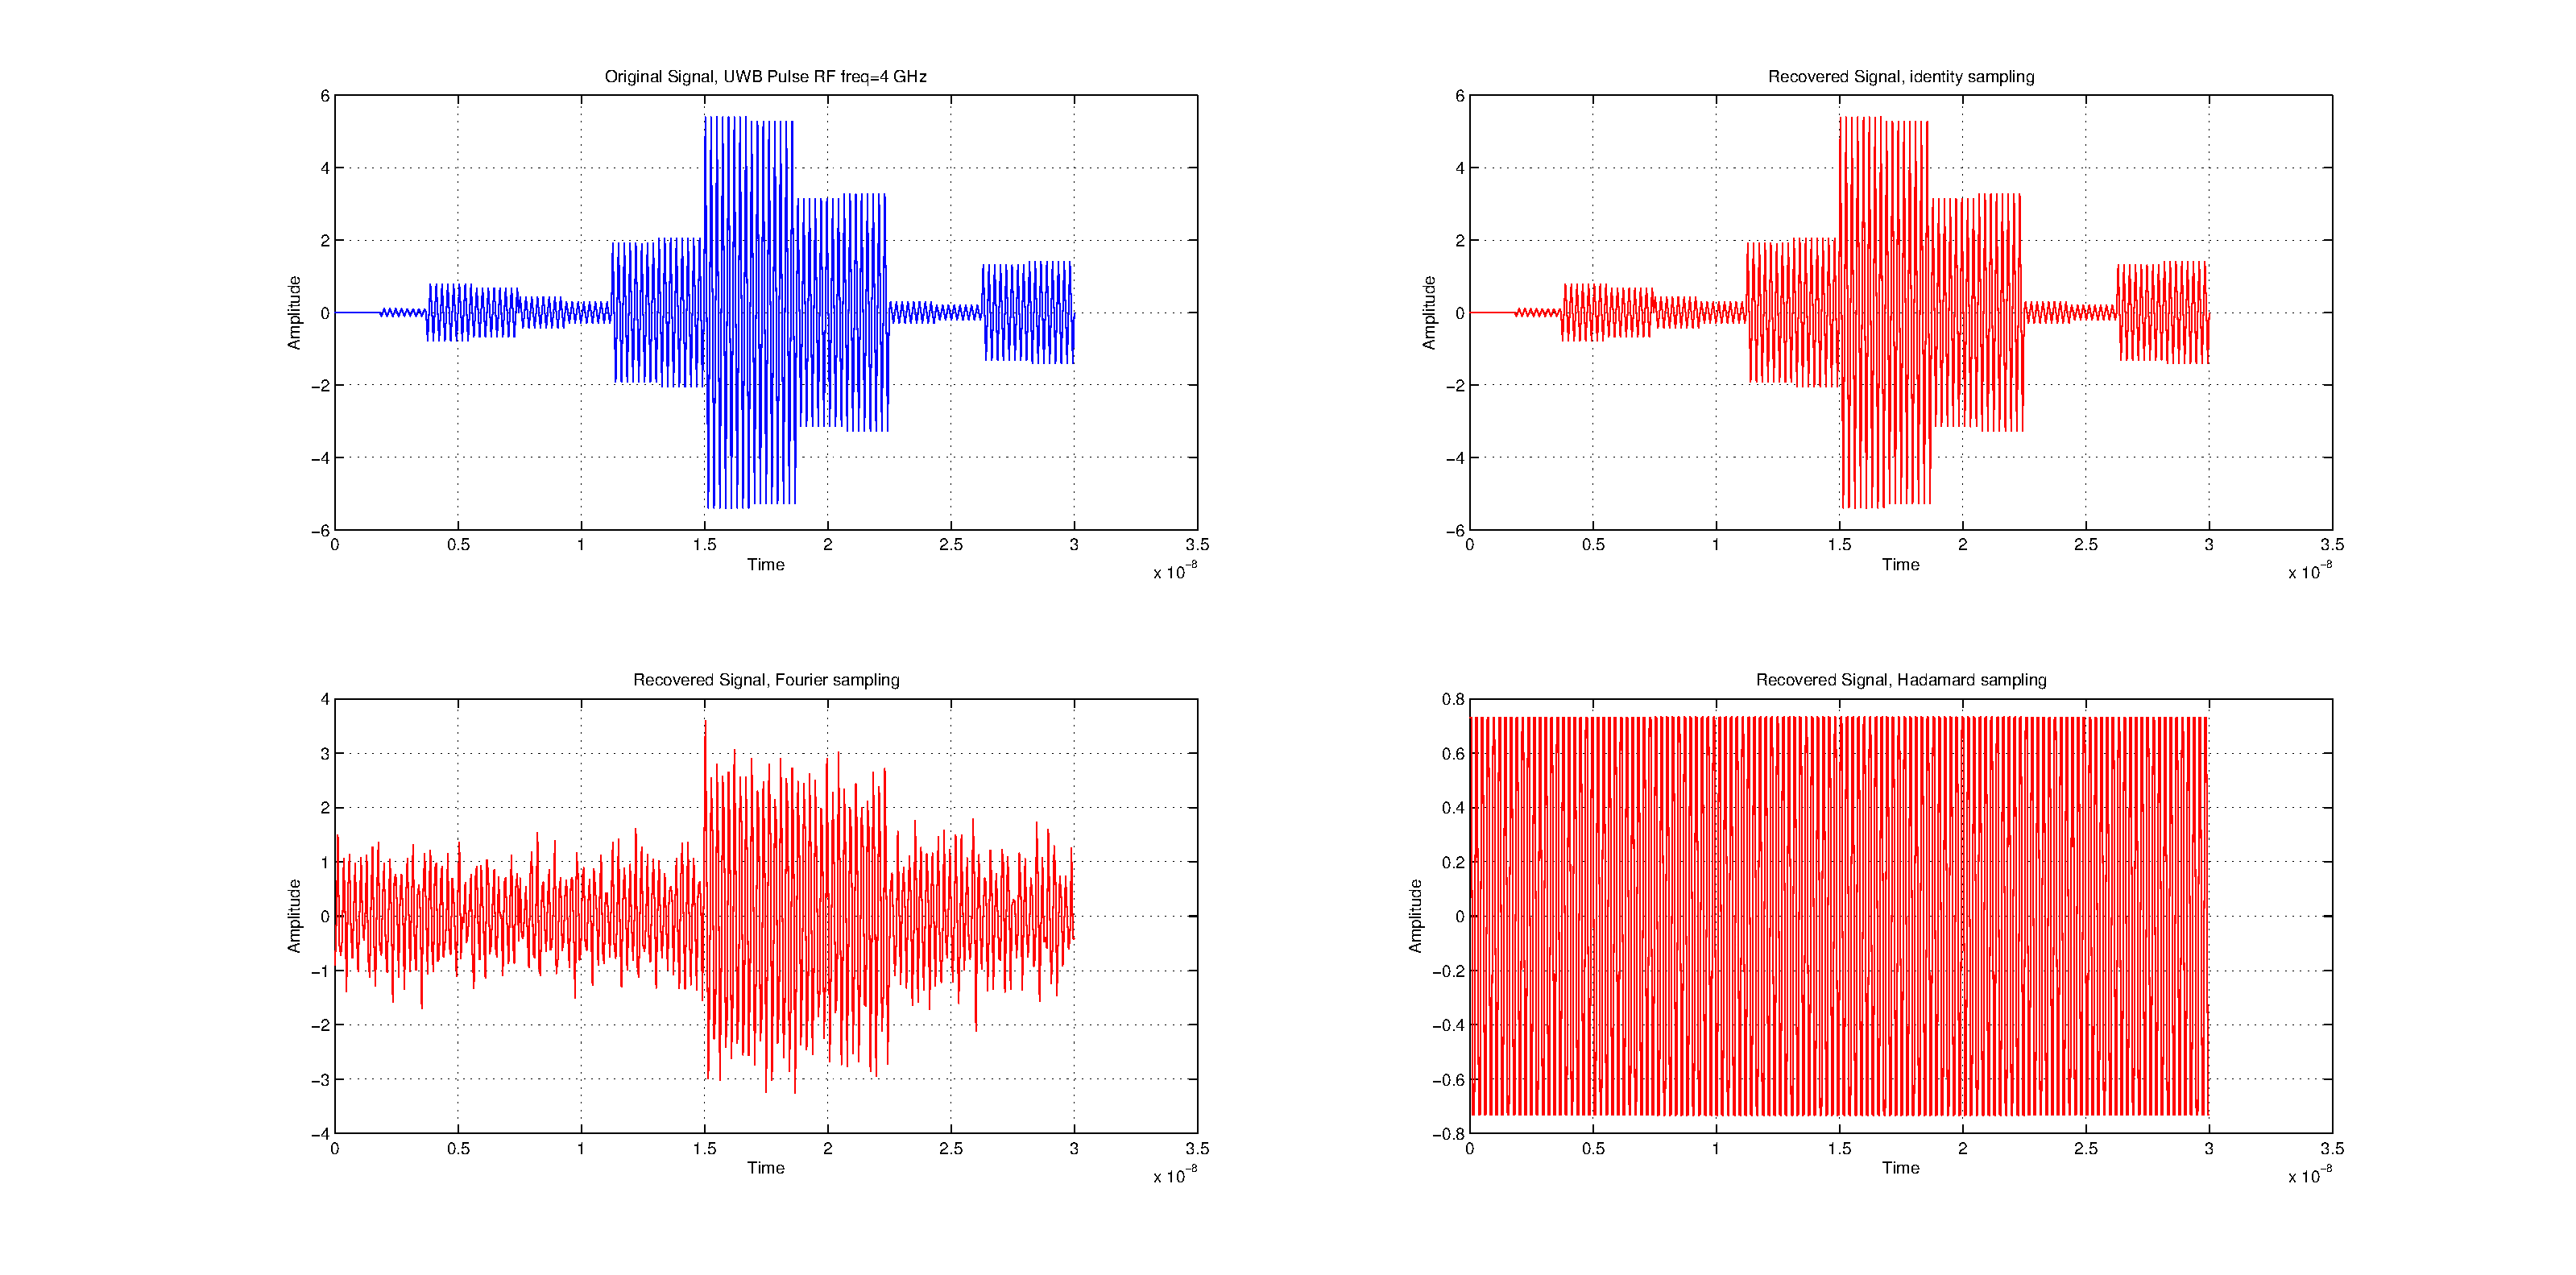
\includegraphics[width=1\textwidth]{figs/incoherence.pdf}
\end{figure}


\end{frame}

%%%%%%%%%%%%%%%%%%%%%%%%%%%%%%%%%%%%%%
%% Frame
%%%%%%%%%%%%%%%%%%%%%%%%%%%%%%%%%%%%%%
\begin{frame}[t]
\frametitle{Incoherence}
\framesubtitle{~~}  %% needed for proper positioning of the logo ...

From Romberg (2008), we have the result:\\

\textbf{Lemma 3.1:} \textit{Let $\boldsymbol{\Phi}$ be an arbitrary fixed orthogonal matrix
, and create $H$ at random with $H = N^{-\frac{1}{2}} F^* \Sigma F$. Choose $0<\delta<1$.
Then with probability exceeding $1-\delta$, the coherence $\mu(H,\boldsymbol{\Phi})$ 
will obey} \\
\begin{equation}
	\mu(H,\boldsymbol{\Phi}) \leq 2 \sqrt{\log \left(\frac{2N^2}{\delta} \right)}
	\label{incoherence_bd1}
\end{equation}
\\
Our random basis is incoherent to \textbf{any} basis with a high probability!

\end{frame}



%%%%%%%%%%%%%%%%%%%%%%%%%%%%%%%%%%%%%%
%% Frame
%%%%%%%%%%%%%%%%%%%%%%%%%%%%%%%%%%%%%%
\begin{frame}[t]
\frametitle{Incoherence}
\framesubtitle{~~}  %% needed for proper positioning of the logo ...

From Do et al (2012), we have the result:\\

\textbf{Theorem III.3:} \textit{Given $F$ and $R$ as defined above, let $A=FR$, and $\Phi$ a fixed orthogonal matrix. Then if the magnitude of the entries of $F$ are bounded by $\mathcal{O}(\frac{1}{\sqrt{B}})$, we have that}
\begin{equation}
	\mu(A,\Phi) \leq \mathcal{O}\left(\sqrt{\frac{\log{\frac{N}{\delta}}}{B}}\right)
\end{equation}
Additionally, if the maximal entry of $\Phi$ (the sparsity domain) is $\mathcal{O}\left(\frac{1}{\sqrt{N}}\right)$,
we can change the bound to 
\begin{equation}
	\label{incoherence_bd2}
	\mu(A,\Phi) \leq \mathcal{O} \left( \sqrt{\frac{\log{\frac{N}{\delta}}}{N}}\right)
\end{equation}

\end{frame}


%%%%%%%%%%%%%%%%%%%%%%%%%%%%%%%%%%%%%%
%% Frame
%%%%%%%%%%%%%%%%%%%%%%%%%%%%%%%%%%%%%%

\begin{frame}[t]
\frametitle{Matrix Type and Error}
\framesubtitle{~~}  %% needed for proper positioning of the logo ...




\begin{table}[h]
\begin{tabular}{lll|lllll}
	\textbf{Matrix Type}       & \textbf{Input Randomizer} & \textbf{Output Randomizer} & \textbf{Error} & \textbf{Time} & \\ \hline
	\multirow{2}{*}{Circulant} & \multirow{2}{*}{N/A}      & Sub                   & 0.0156         & 4.97s         & \\
	                           &                           & RPMS                  & 0.0159         & 7.80s         & \\
\end{tabular}
\end{table}

\begin{table}[h]
\begin{tabular}{lll|lllll}
	\textbf{Matrix Type}      & \textbf{Input Randomizer} & \textbf{Output Randomizer} & \textbf{Error} & \textbf{Time} & \\ \hline
	\multirow{2}{*}{Toeplitz} & \multirow{2}{*}{N/A}      & Sub                   & 0.0193         & 25.9s         & \\
	                          &                           & RPMS                  & 0.0170         & 16.9s         & \\
\end{tabular}
\end{table}

\end{frame}


%%%%%%%%%%%%%%%%%%%%%%%%%%%%%%%%%%%%%%
%% Frame
%%%%%%%%%%%%%%%%%%%%%%%%%%%%%%%%%%%%%%

\begin{frame}[t]
\frametitle{Matrix Type and Error}
\framesubtitle{~~}  %% needed for proper positioning of the logo ...


\begin{table}[h]
\begin{tabular}{lll|lllll}
	\textbf{Matrix Type}     & \textbf{Input Randomizer} & \textbf{Output Randomizer} & \textbf{Error} & \textbf{Time } & \\ \hline
	\multirow{4}{*}{Fourier} & \multirow{2}{*}{Local}    & Sub                        & 0.0183         & 7.89s          & \\
	                         &                           & RPMS                       & 0.0517         & 14.0s          & \\
	                         & \multirow{2}{*}{Global}   & Sub                        & 0.0166         & 4.98s          & \\
	                         &                           & RPMS                       & 0.0529         & 14.1s          & \\
\end{tabular}
\end{table}

\begin{table}[h]
\begin{tabular}{lll|lllll}
	\textbf{Matrix Type}      & \textbf{Input Randomizer} & \textbf{Output Randomizer} & \textbf{Error} & \textbf{Time } & \\ \hline
	\multirow{4}{*}{Hadamard} & \multirow{2}{*}{Local}    & Sub                        & 0.0167         & 552s           & \\
	                          &                           & RPMS                       & 0.0153         & 752s           & \\
	                          & \multirow{2}{*}{Global}   & Sub                        & 0.0157         & 544s           & \\
	                          &                           & RPMS                       & 0.0137         & 782s           & \\
\end{tabular}
\end{table}


\end{frame}

%%%%%%%%%%%%%%%%%%%%%%%%%%%%%%%%%%%%%%
%% Frame
%%%%%%%%%%%%%%%%%%%%%%%%%%%%%%%%%%%%%%

\begin{frame}[t]
\frametitle{Timing}
\framesubtitle{~~}  %% needed for proper positioning of the logo ...


\begin{table}[h]
\begin{tabular}{l|lllllll}
	\textbf{Matrix Type} & Gaussian & Circulant & Toeplitz & Fourier & Hadamard \\ \hline
	\textbf{Time}        & 12.2s    & 1.65s     & 4.24s    & 1.50s   & 102s*    \\
\end{tabular}
\end{table}
* The fast Walsh-Hadamard transform in \textsc{Matlab} is written in \textsc{Matlab} and is slow.


\end{frame}


%%%%%%%%%%%%%%%%%%%%%%%%%%%%%%%%%%%%%%
%% Frame
%%%%%%%%%%%%%%%%%%%%%%%%%%%%%%%%%%%%%%
\begin{frame}[t]
	\frametitle{Our contributions}
	\framesubtitle{~~}  %% needed for proper positioning of the logo ...

	Our work can be summarized as follows
	\begin{itemize}
		\item We have combined the structures Do et al. (2012) and the subsampling operator 
			of Romberg (2008) to propose a new type of structured random matrix which offers 
			comprable practical performance
		\item We implemented a randomized Toeplitz matrix that built on the random structure
			used by Romberg (2008) for circulant matrices by expanding the system to size $2N$.
	\end{itemize}

\end{frame}



%%%%%%%%%%%%%%%%%%%%%%%%%%%%%%%%%%%%%%
%% Frame
%%%%%%%%%%%%%%%%%%%%%%%%%%%%%%%%%%%%%%
\begin{frame}[t]
	\frametitle{Future work}
	\framesubtitle{~~}  %% needed for proper positioning of the logo ...

	Looking ahead, we have the following questions for areas of future research
	\begin{itemize}
		\item We would like to see empirically how sparsity affects each of the methods we 
			have looked at to compare with the theory (comparing to the $S\log{N}$ bound. In 
			Yin et al (2010), they had some results, but not for most of the matrices we 
			compared here. 
		\item We did most minimizations in the $TV$ norm, but we would like to see an 
			implementation of an ADMM (alternating direction method of multipliers) on an
			objective function containing both the $L_1$ and the $TV$ norms. Yin et al (2010)
			implemented this, but not with the randomizations discussed here. 
	\end{itemize}

\end{frame}

%%%%%%%%%%%%%%%%%%%%%%%%%%%%%%%%%%%%%%
%% Frame
%%%%%%%%%%%%%%%%%%%%%%%%%%%%%%%%%%%%%%
\begin{frame}[t]
	\frametitle{Thank you}
	\framesubtitle{~~}  %% needed for proper positioning of the logo ...
	Questions?
\end{frame}



\end{document}


